\chapter{Results}
\lhead{\chaptername~\thechapter. \emph{Spherical SfM}}
In this chapter, we comment the results obtained with our SfM pipeline.
We tested our approach with both computer-generated and real-world environments.
We compare the pose estimation results with ground truth in the synthetic cases
while we only give a qualitative evaluation for the multi-view stereo
reconstruction step for both the synthetic and real video sequences.
We implemented our pipeline in MATLAB R2017a, and we collected our results using
a computer equipped with an Intel i5-2400 at 3.10 GHz and 12 GB of RAM.

\section{Datasets Description}
\subsection{Synthetic Scenes}
The first computer-generated environment is a 3D simple scene that we created in Blender 2.78c.
This scene is composed of a room with 5 polyhedrons. We added some image textures to both
room's walls and shapes'faces to increase matching inliers.
The camera moves on a continuous curve around the polyhedrons and both its
position and orientation change.
Figure~\ref{fig:test6} shows some rendered images for this environment.
%
\begin{figure}
\centering
	\begin{subfigure}{0.4\textwidth}
		\centering
		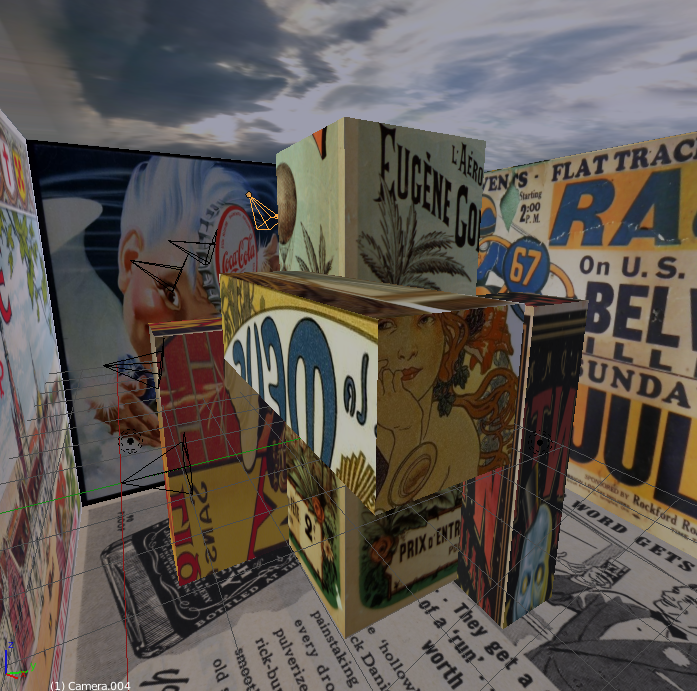
\includegraphics[width=\textwidth]{img/test6_1}
	\end{subfigure}
    %
	\begin{subfigure}{0.4\textwidth}
		\centering
		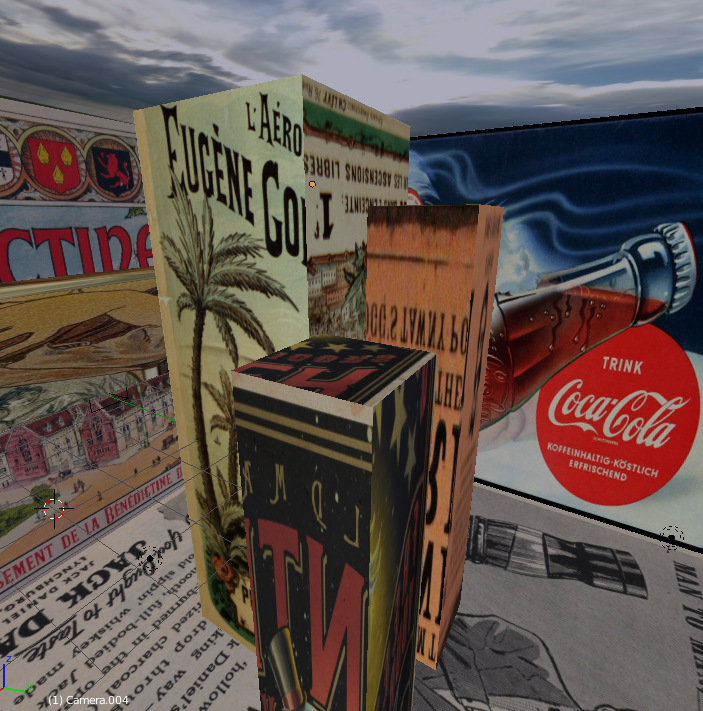
\includegraphics[width=\textwidth]{img/test6_2}
	\end{subfigure}
    %
	\begin{subfigure}{0.4\textwidth}
		\centering
		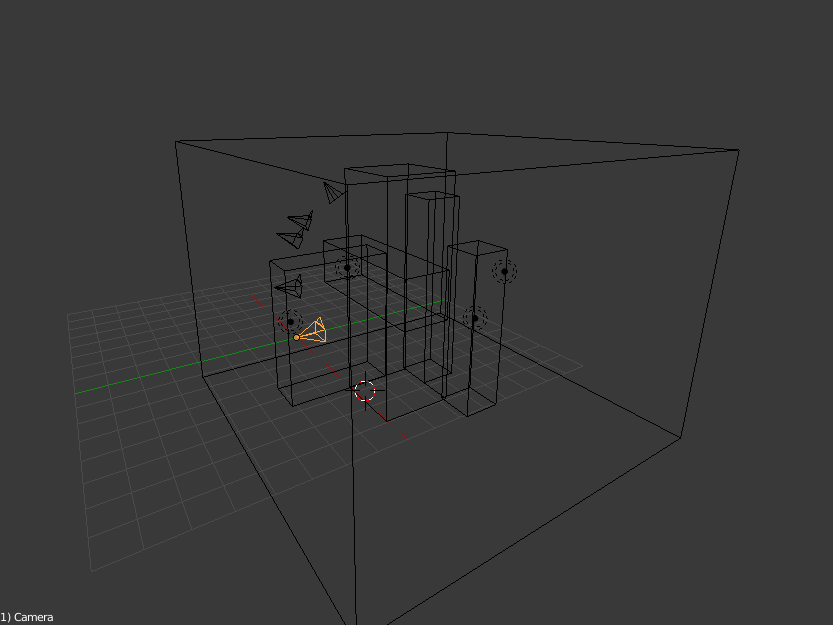
\includegraphics[width=\textwidth]{img/test6_3}
	\end{subfigure}
    %
	\begin{subfigure}{0.4\textwidth}
		\centering
		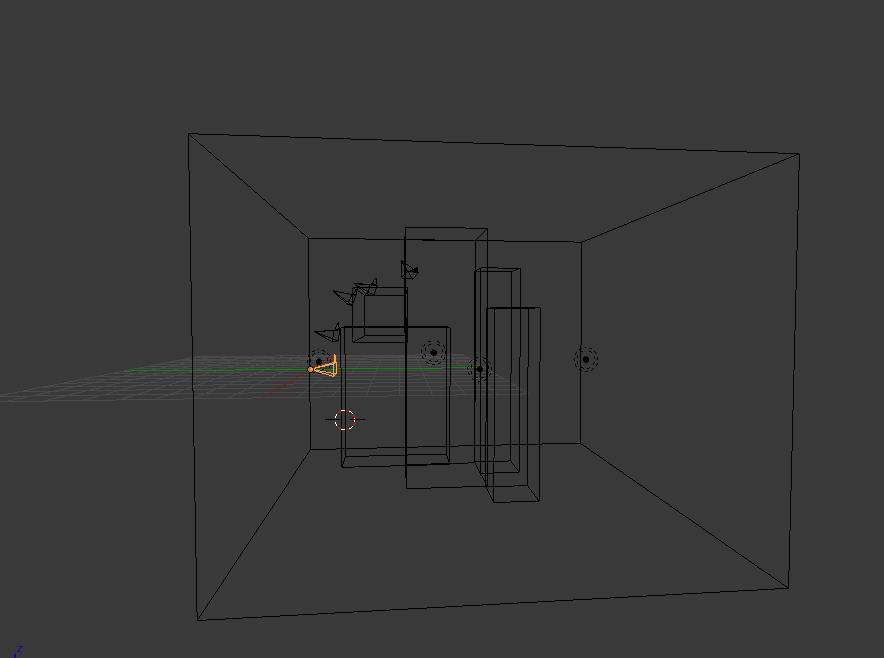
\includegraphics[width=\textwidth]{img/test6_4}
	\end{subfigure}
	%
	\begin{subfigure}{0.8\textwidth}
		\centering
		\includegraphics[width=\textwidth]{img/test6_5}
	\end{subfigure}
	%
	\caption{The first computer-generated environment that we used in our tests and
	an example equirectangular image from this scene: two views of the scene (top row),
	wireframe visualizations of the same scene (middle row), and an example
	equirectangular image produced with this setup (bottom).}
    \label{fig:test6}
\end{figure}
%

In the second computer-generated scene, we recreated a town square surrounded by
a covered walkway (i.e., \emph{loggia}). The roof of the walkway is supported by columns on the inner
side, the one that is oriented toward the square's centre, and by a wall on the
outer side.
Again the environment is contained in a room and every surface is textured.
The camera moves along the walkway with a non-uniform speed while pointing toward
the centre of the square. Figure~\ref{fig:test_square} shows some images
for this second environment.
%
\begin{figure}
\centering
	\begin{subfigure}{0.4\textwidth}
		\centering
		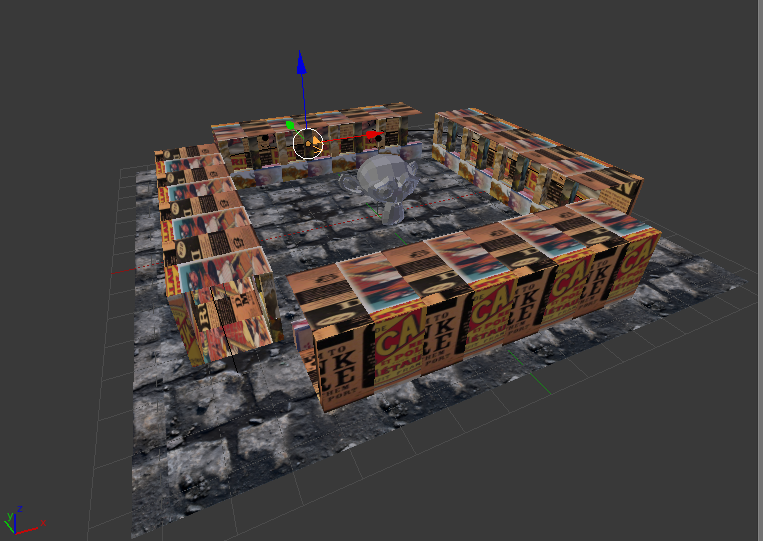
\includegraphics[width=\textwidth]{img/square1}
	\end{subfigure}
    %
	\begin{subfigure}{0.4\textwidth}
		\centering
		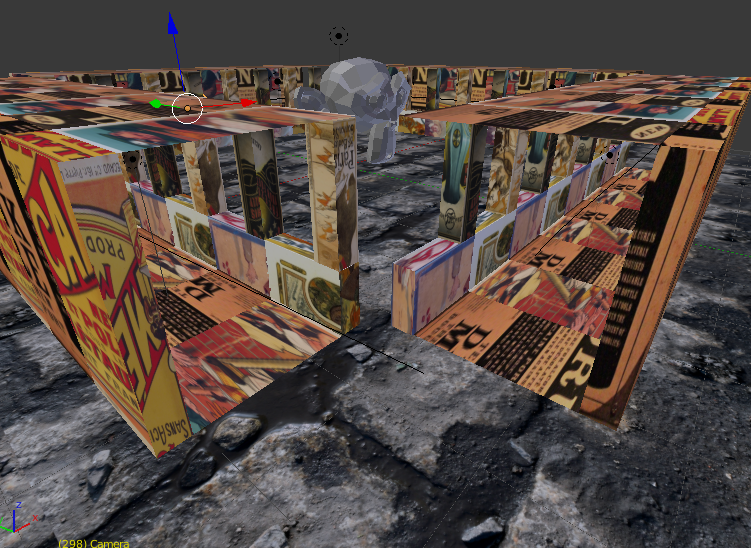
\includegraphics[width=\textwidth]{img/square2}
	\end{subfigure}
    %
	\begin{subfigure}{0.8\textwidth}
		\centering
		\includegraphics[width=\textwidth]{img/square3}
	\end{subfigure}
    %
	\begin{subfigure}{0.8\textwidth}
		\centering
		\includegraphics[width=\textwidth]{img/square4}
	\end{subfigure}
	%
	\caption{The computer-generated town square environment: two views of the
	model (top row) and two examples of equirectangular images produced from this
	scene (middle and bottom).}
    \label{fig:test_square}
\end{figure}

\subsection{Real environment}\label{subsec:real_environment}
We tested our pipeline with a real video footage too. In this case, 
we do not have the ground truth
for the camera poses. However, the quality of the
reconstruction is a good indicator of the pipeline performance.
We captured the real-world sequence with a Ricoh Theta S camera in a town square
surrounded by a \emph{loggia}. As before, we walked around the square, along the covered
walks, keeping the camera above the user's head using a stick.
The user does not influence the camera poses estimation because it appears in the
pole region of the image sphere and, as we said in
Section~\ref{sec:pipeline_pose_estimation}, we discard potential matches in
these areas.
We present some pictures of the real-wolrd environment together with some examples
of the equirectangular images of the town square in
Figure~\ref{fig:piazzaLeoni}.
%
\begin{figure}[h]
\centering
	\begin{subfigure}{0.7\linewidth}
		\centering
		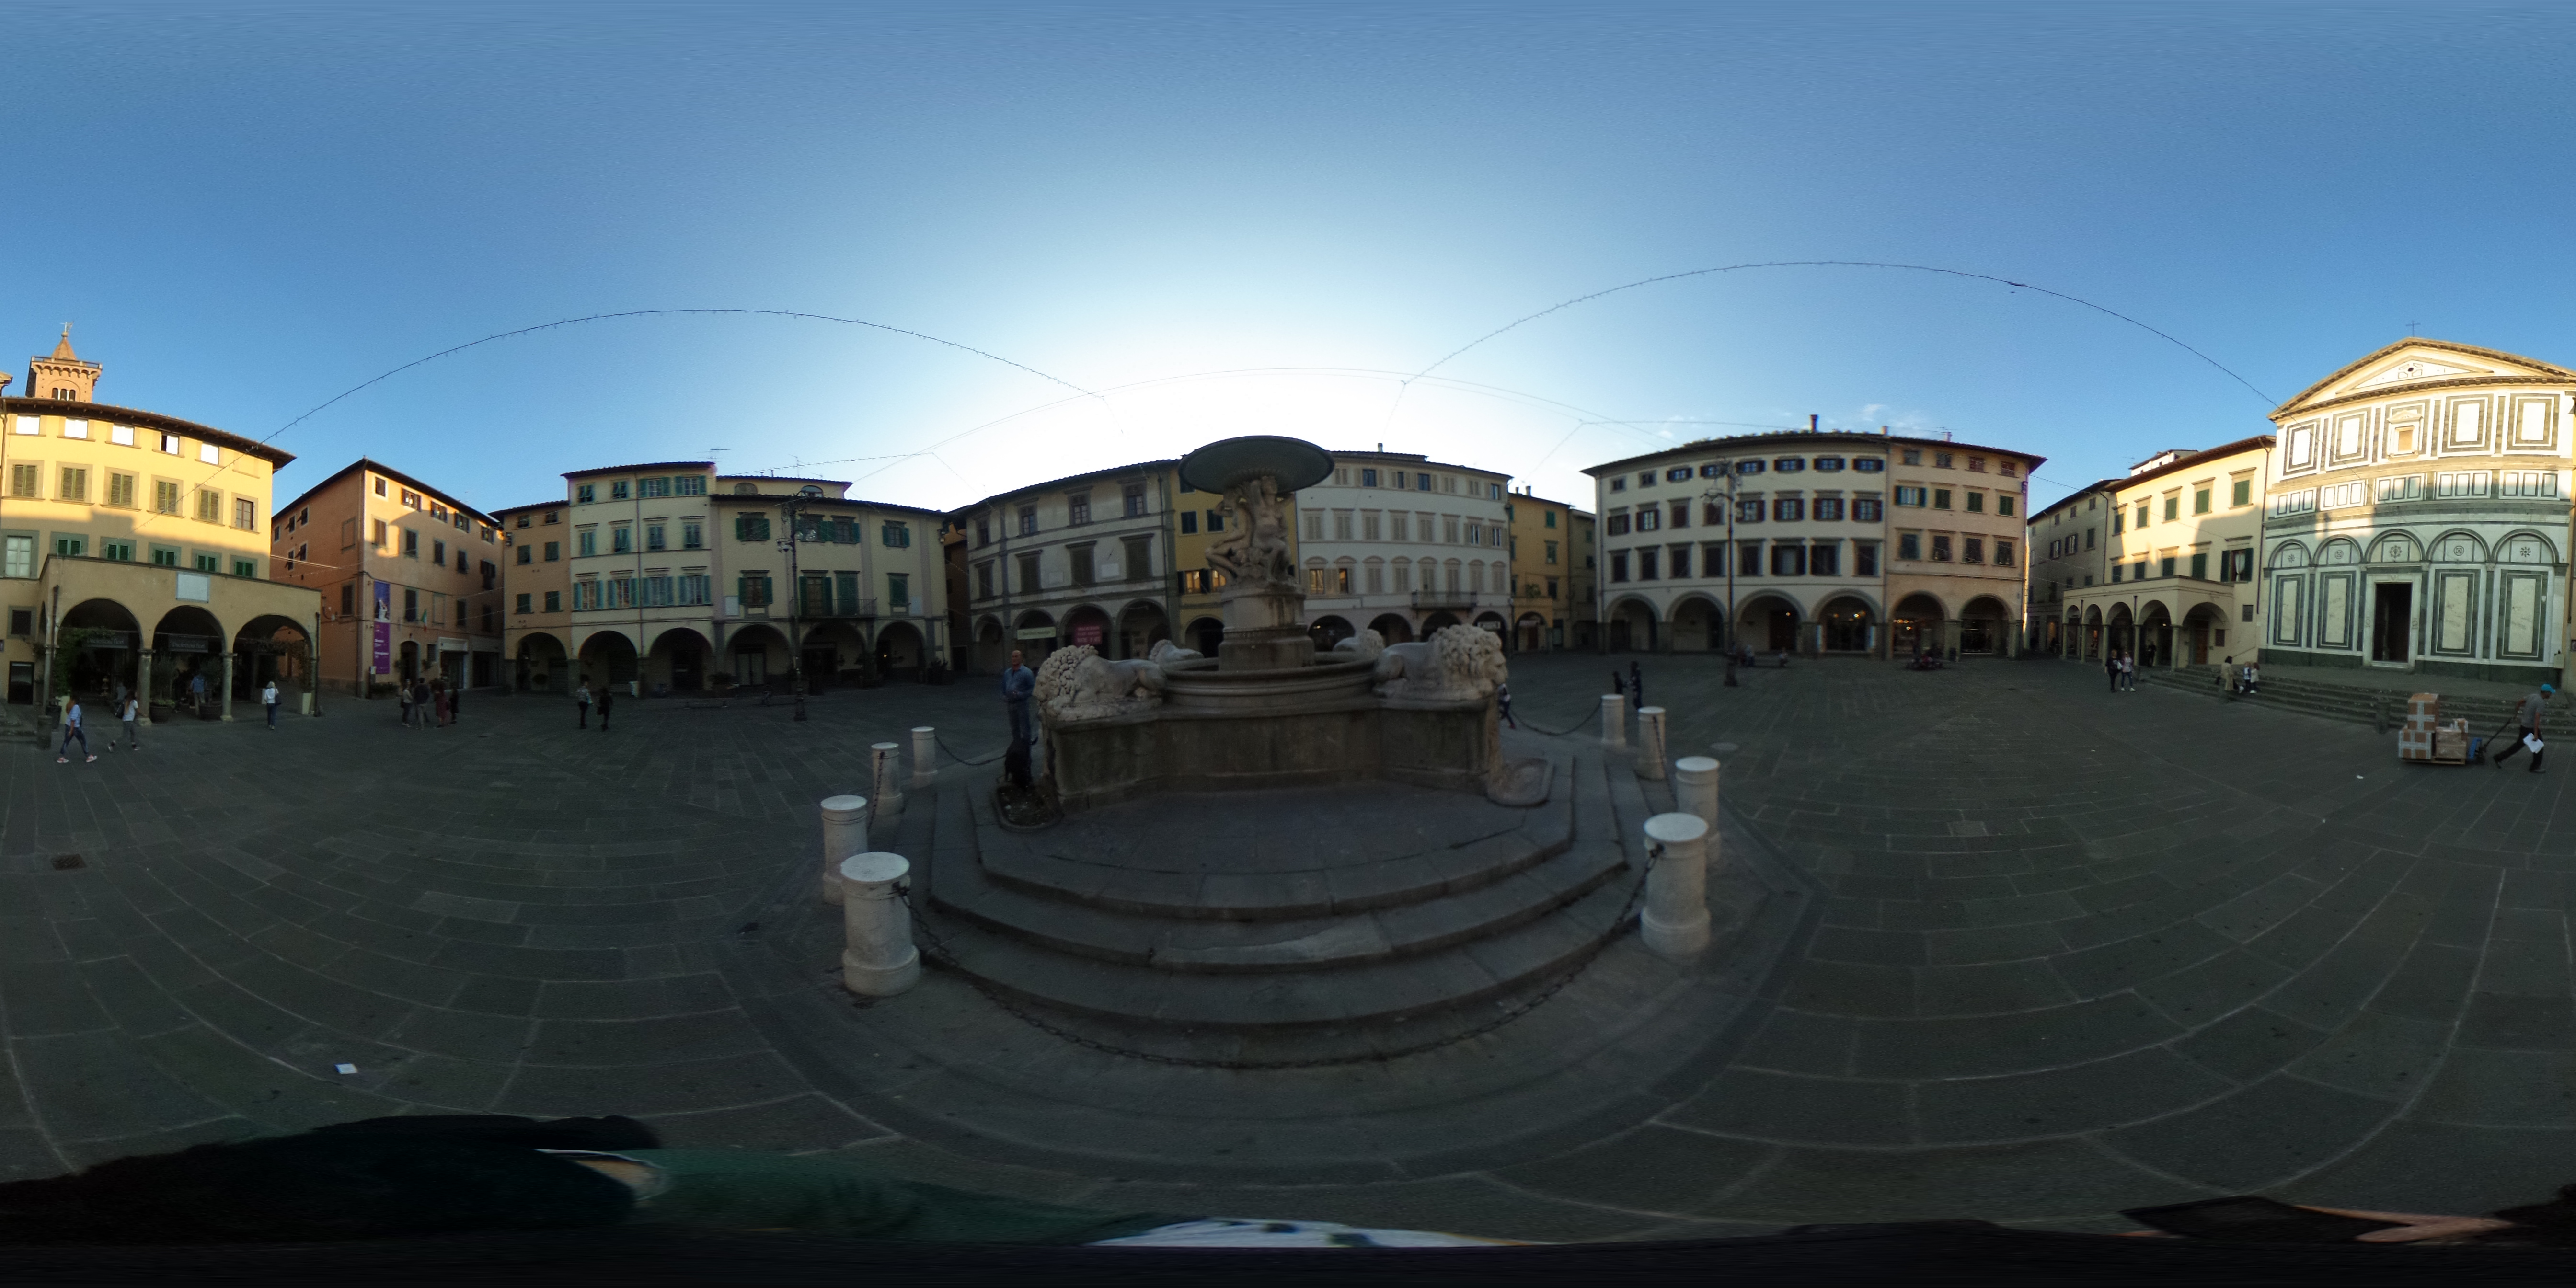
\includegraphics[width=\linewidth]{img/piazzaLeoni.jpg}
		\caption{Panoramic view of the real town square.}
	\end{subfigure}
	%
	\begin{subfigure}{0.7\linewidth}
		\centering
		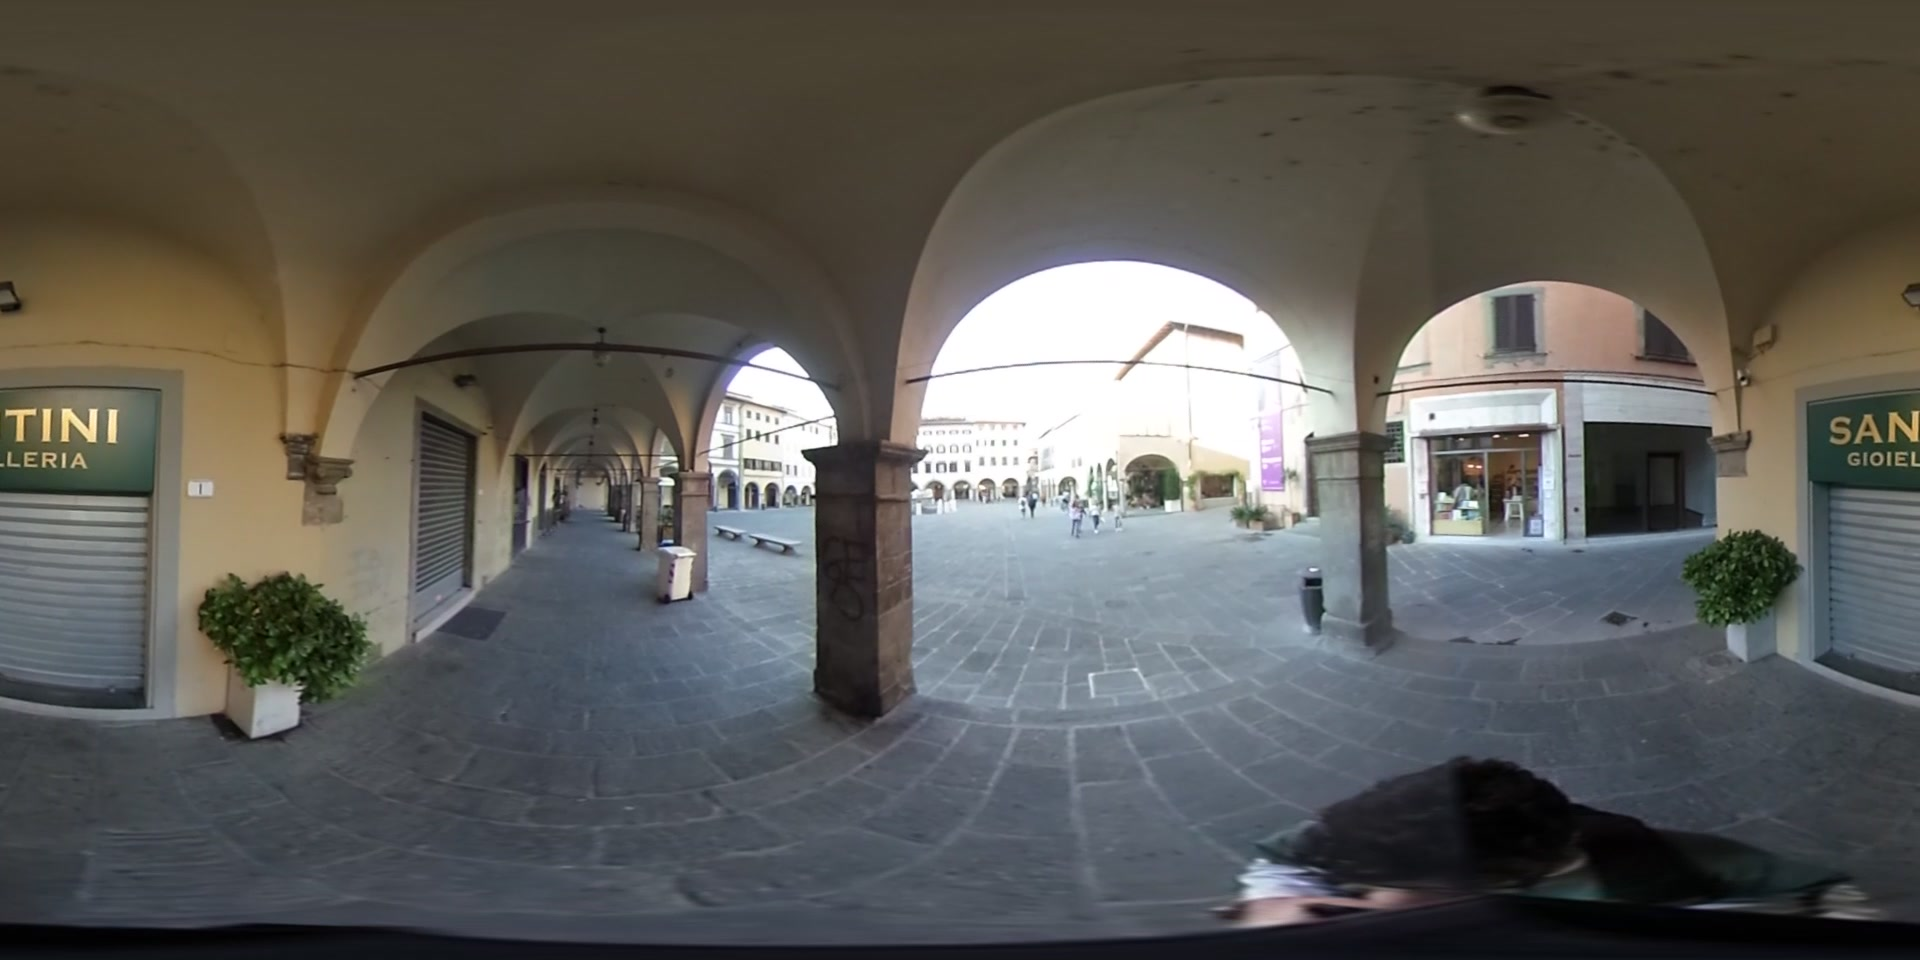
\includegraphics[width=\linewidth]{img/piazzaLeoni_exampleds.jpg}
		\caption{Example frame from the real town square sequence.}
	\end{subfigure}
\caption{The town square we used in our real-world reconstruction test.}
\label{fig:piazzaLeoni}
\end{figure}

\section{Experiment Results}
\subsection{Window Size Test}
We performed an experiment to choose the optimal window size for the proposed windowed
bundle adjustment (Section~\ref{subsec:windowed_ba}). In this experiment, we
used the synthetic town square and computed the sum of absolute pose error. In
particular, we consider the location and orientation errors for the estimated poses.
Figure~\ref{fig:sumAbsLocError} shows the comparison of the resulted location error for 20
estimated poses with respect to several windowed and non-windowed adjustment
techniques.
In particular, we can see that the pose error is minimal when we employ the
windowed bundle adjustment with a window that contains five poses at a time.
Windows smaller than five do not bring substantial improvements (as we pointed out in
Section~\ref{subsec:windowed_ba}; to maintain the proper scale, we keep the two poses
in a window fixed), while the error also increases
for larger windows. The performance deterioration when using larger windows
is due to the fact that the windowed adjustment may suffer from the high number
of views to be optimized: if a series of views with wrong estimated poses are
already inside the window and a new pose enters it, the prevalent number of
low-quality estimation may result in the last pose to be aligned to the wrong trajectory
of the previous estimations. Due to this phenomenon, all next views
may be incorrectly optimized. This reduces the performance of the overall
pose estimation.
%
\begin{figure}[h]
\centering
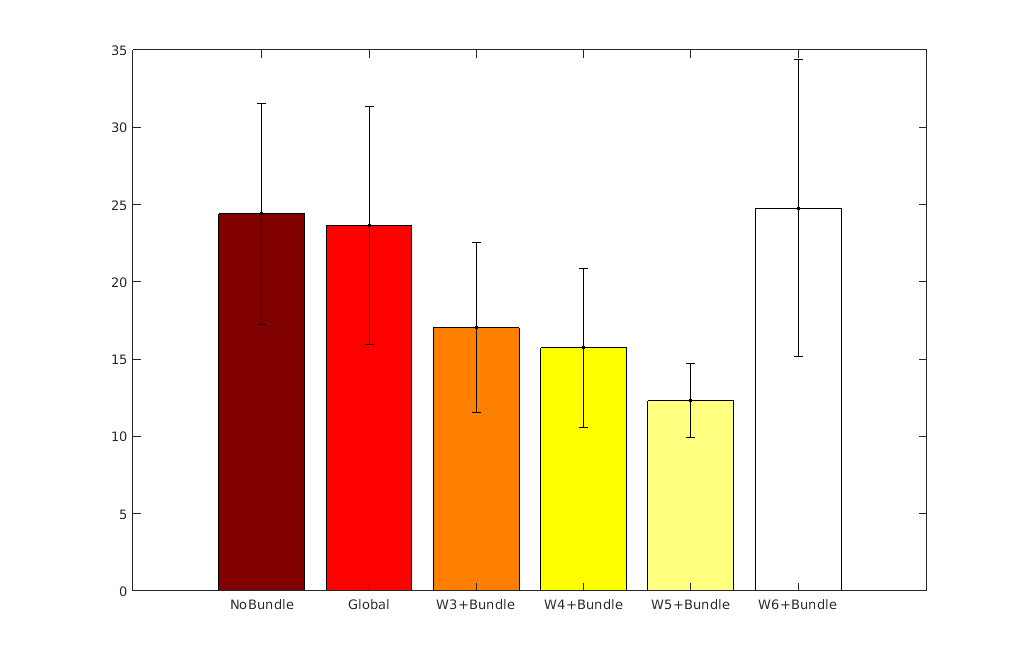
\includegraphics[width=\linewidth]{img/sumAbsLocError.png}
\caption{Location error with respect to different global refinement techniques. The proposed windowed bundle adjustment with a window of size 5 gives the best performance. This choice is optimal also for the orientation
error.}
\label{fig:sumAbsLocError}
\end{figure}

\subsection{Essential Matrix Estimation Test}\label{subsec:essential_test}
In Section~\ref{subsec:essential_estimation}, we said that our pipeline
calls the essential matrix estimation routine until the fraction of inliers
drops below a threshold. In Figure~\ref{fig:essential_test}, we show the
results of an experiment where we compare three different essential matrix
evaluation approaches. The input data for this experiment is composed of
a set of manually selected frames from the first synthetic environment.
The reason why we select the frames is that we do not want this results to be
influenced by the frame filter.
%
\begin{figure}[h]
\centering
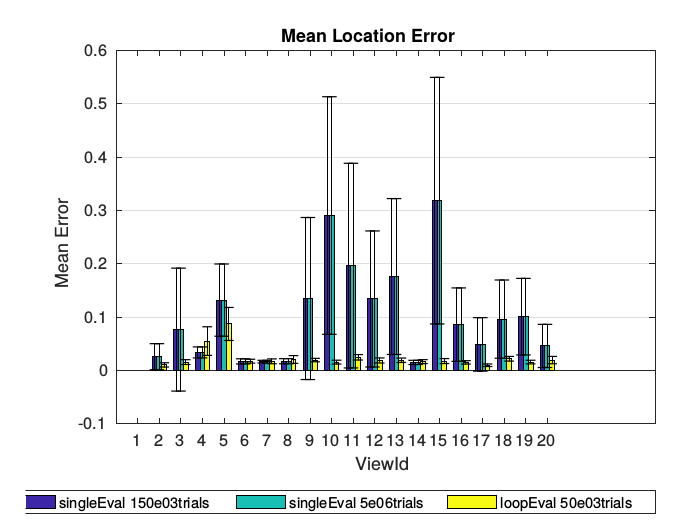
\includegraphics[width=\linewidth]{img/essentialEstimation.png}
\caption{How the location error changes with respect to different essential
matrix estimation function approaches: the purple and light blue columns
represent the average location error results for each frame when the
essential estimation is performed with a single call to the routine, while the
yellow column represent the location error when we perform the estimation
again when the fraction of inliers is too low.}
\label{fig:essential_test}
\end{figure}

\subsection{SfM Phase Result}
In this test, we analyzed the overall results of the initial step of our
pipeline, the motion estimation phase. We used the 365 rendered frames of our
synthetic town square environment. Figure~\ref{fig:trajectory} shows the actual
and estimated trajectory of the camera in the synthetic environment.
%
\begin{figure}[h]
\centering
\begin{subfigure}{0.45\linewidth}
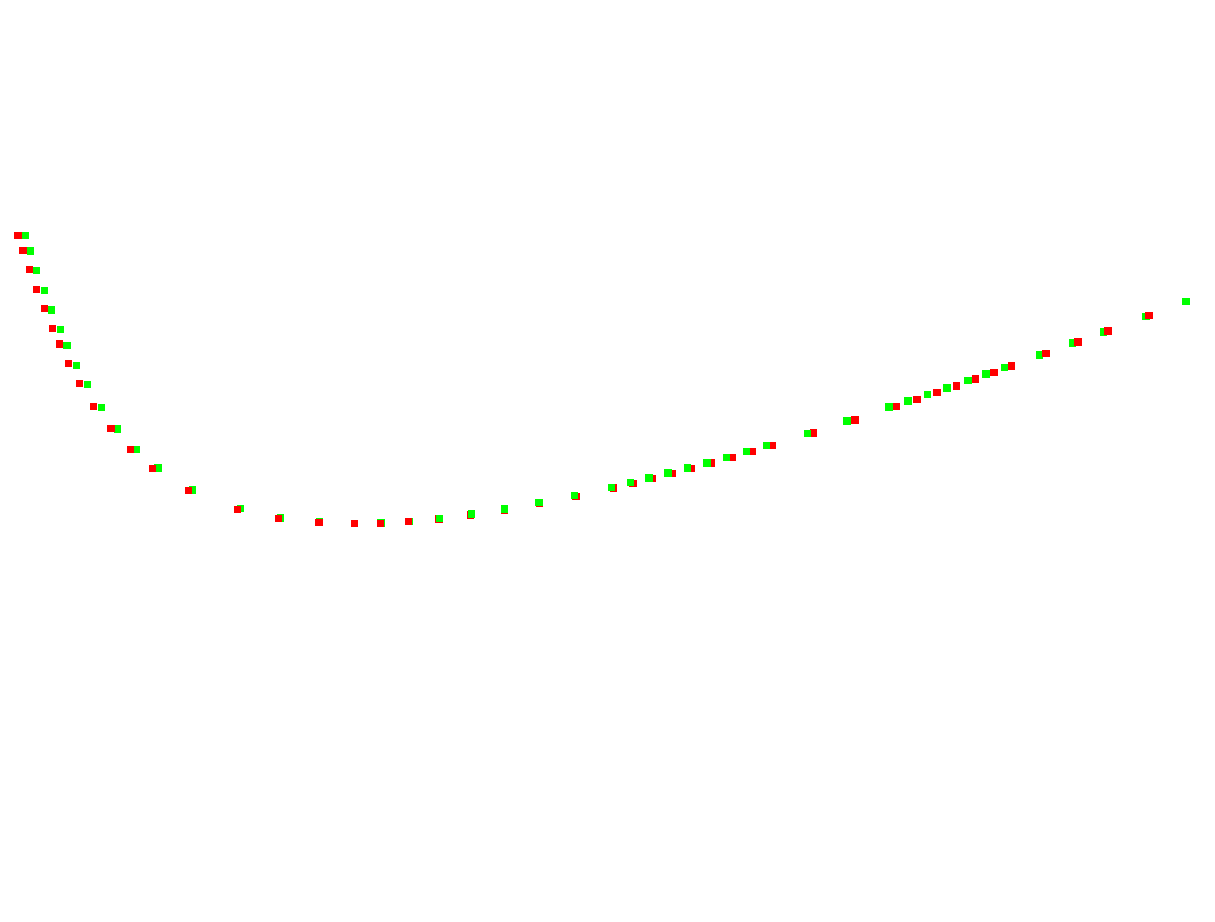
\includegraphics[width=\linewidth]{img/snapshot00.png}
\caption{Camera's trajectory (green) with ground truth (red).}
\label{fig:trajectory1}
\end{subfigure}
\begin{subfigure}{0.45\linewidth}
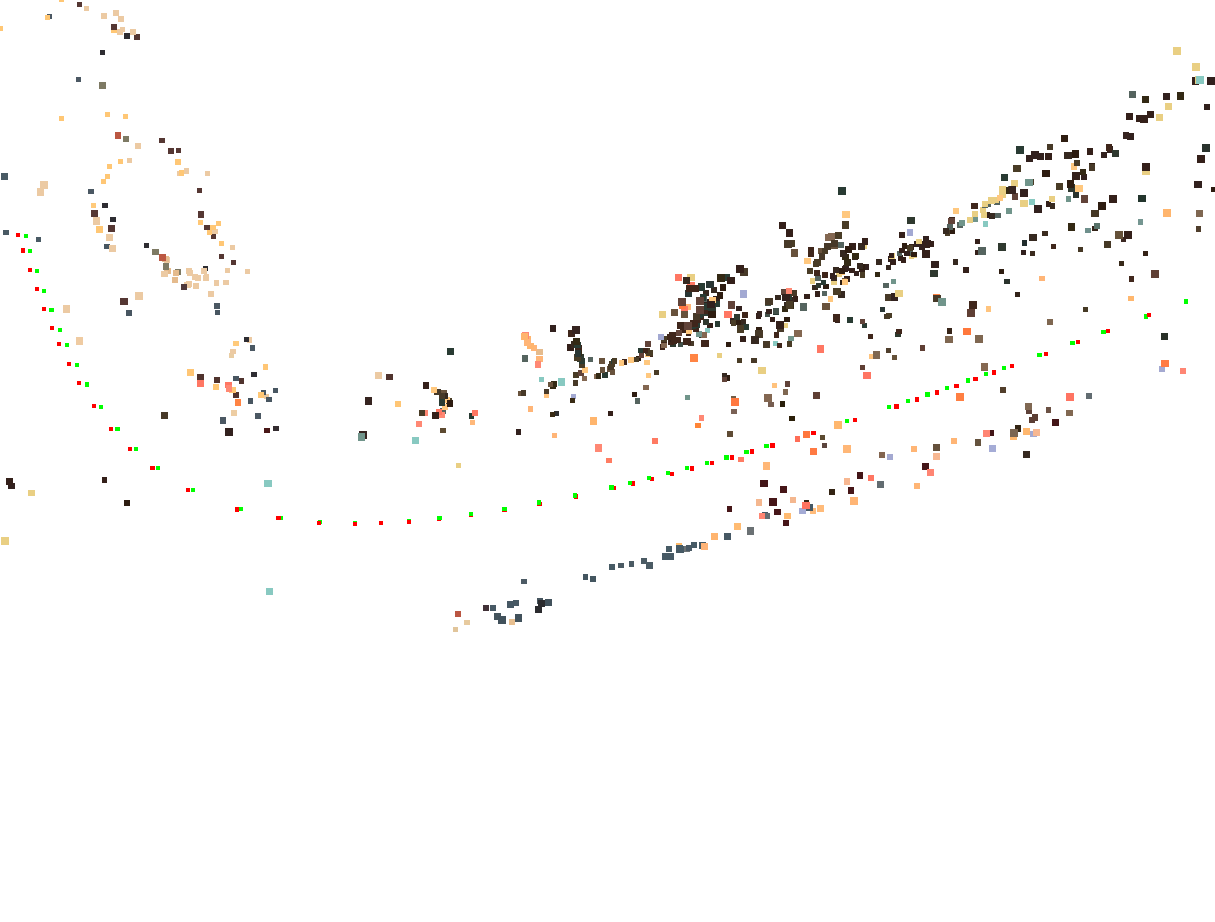
\includegraphics[width=\linewidth]{img/snapshot01.png}
\caption{Camera's trajectory and sparse point cloud.}
\label{fig:trajectory2}
\end{subfigure}
\begin{subfigure}{\linewidth}
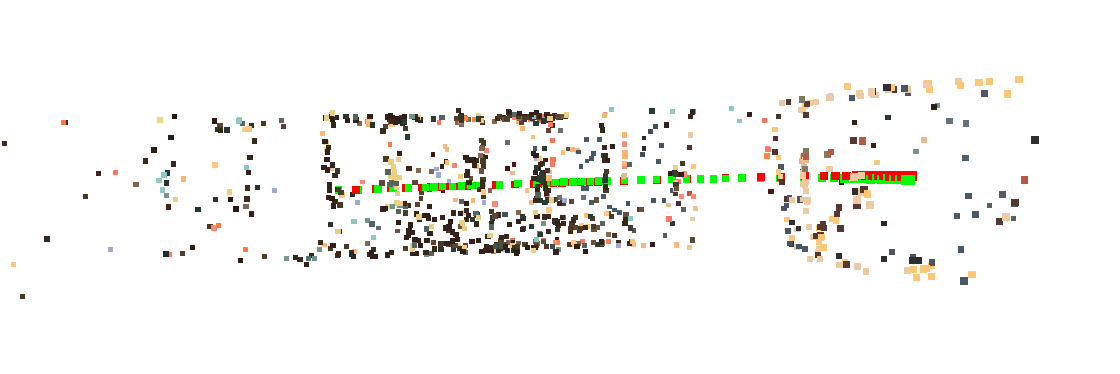
\includegraphics[width=\linewidth]{img/snapshot02.png}
\caption{Another view of the sparse point cloud.}
\label{fig:trajectory3}
\end{subfigure}
\caption{The results of the pose estimation phase: estimated poses (green
points) compard with ground truth (red points) (a); the sparse point cloud
composed of the triangulated features points (b); another view of the sparse
point cloud where we can distinguish the columns of the inner side of the
walkway (c).}
\label{fig:trajectory}
\end{figure}
%
\subsection{Disparity Maps}
Figures~\ref{fig:llDisparity} and \ref{fig:disparity_comparison}
shows an example of disparity map computed
with our adaptive block-matching algorithm and the comparison with
traditional block-matching algorithm. Darker colours refer to the points
with less disparity thus, farther from the camera. On the other hand, the closer
objects have brighter colours.
%
\begin{figure}[h]
\centering
	\begin{subfigure}{\linewidth}
		\centering
		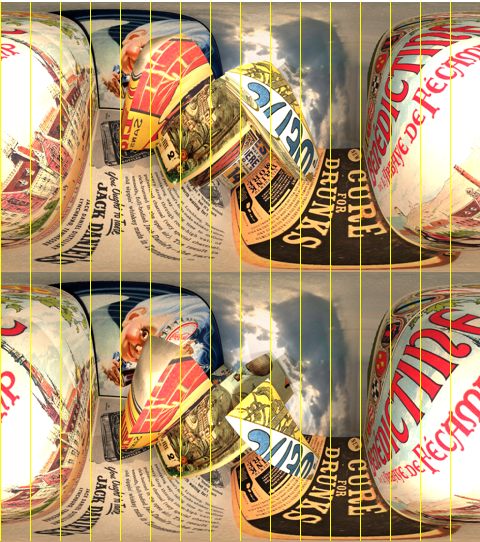
\includegraphics[width=\linewidth]{img/rectified_pair.png}
		\caption{Original rectified pair.}
	\end{subfigure}
	%
	\begin{subfigure}{\linewidth}
		\centering
		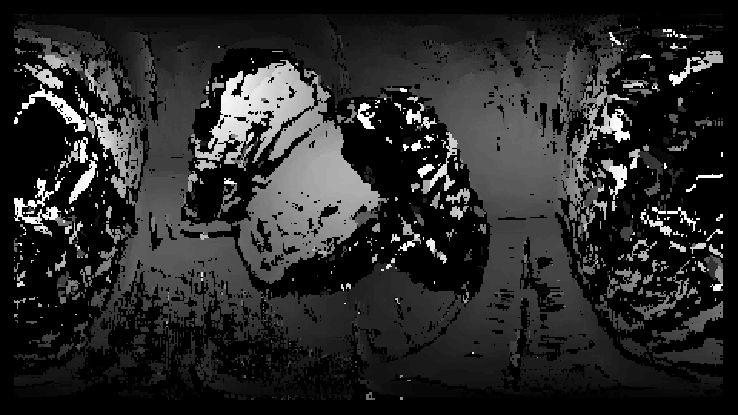
\includegraphics[width=\linewidth]{img/lldisparity2.png}
		\caption{Computed disparity map.}
	\end{subfigure}
\caption{An example of disparity map computed with our adaptive block-matching
algorithm. The black points in the map are points whose disparity is equal to
zero or that are occluded in the other image; in both cases, these points are
not triangulated.}
\label{fig:llDisparity}
\end{figure}
%
\begin{figure}[h]
\centering
	\begin{subfigure}{0.7\linewidth}
		\centering
		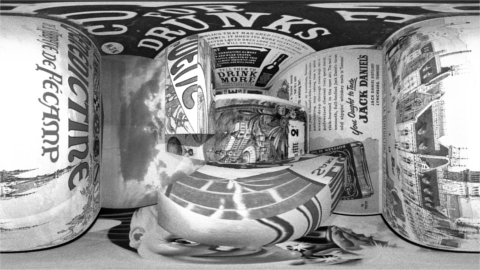
\includegraphics[width=\linewidth]{img/original.png}
		\caption{Original reference image.}
	\end{subfigure}
	%
	\begin{subfigure}{0.7\linewidth}
		\centering
		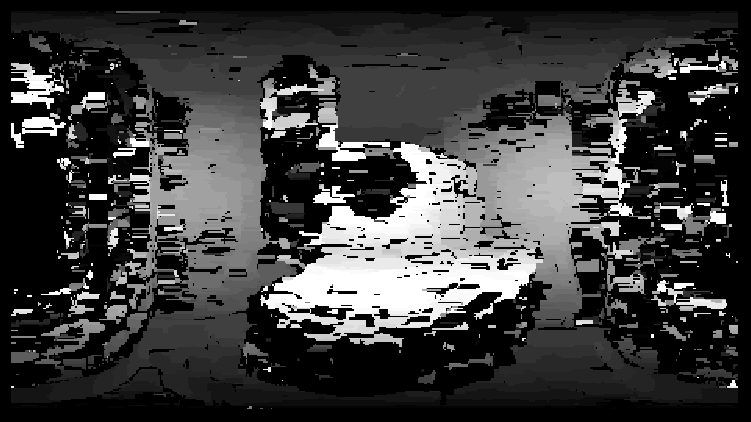
\includegraphics[width=\linewidth]{img/our_disparity.png}
		\caption{The disparity map computed with our adaptive block-matching
		algorithm.}
	\end{subfigure}
	%
	\begin{subfigure}{0.7\linewidth}
		\centering
		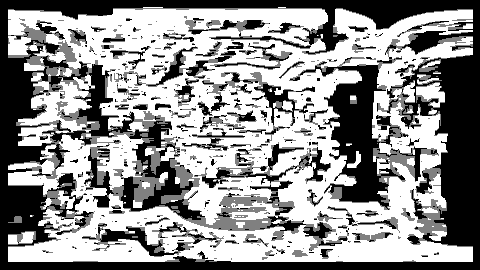
\includegraphics[width=\linewidth]{img/legacy_disparity.png}
		\caption{The disparity map computed with the standard block-matching
		algorithm.}
	\end{subfigure}
\caption{Comparison of our adaptive block-matching algorithm's result (b) with
standard block-matching algorithm (c). The parameters are the same for
both algorithms. We did not perform the cross-check for the last map (c).
The cross-check completely invalidated the maps when adaptive block-matching is
not used.}
\label{fig:disparity_comparison}
\end{figure}
%
\subsection{Environments Reconstruction}
Figure~\ref{fig:real_reconstruction} shows the resulting reconstruction of the
real town square's loggia described in Section~\ref{subsec:real_environment}.
This reconstruction is the result of a video sequence composed of 400 frames;
the frame filter selected 48 frames then used as input data for our pipeline.
%
\begin{figure}[h]
\centering
	\begin{subfigure}{\linewidth}
		\centering
		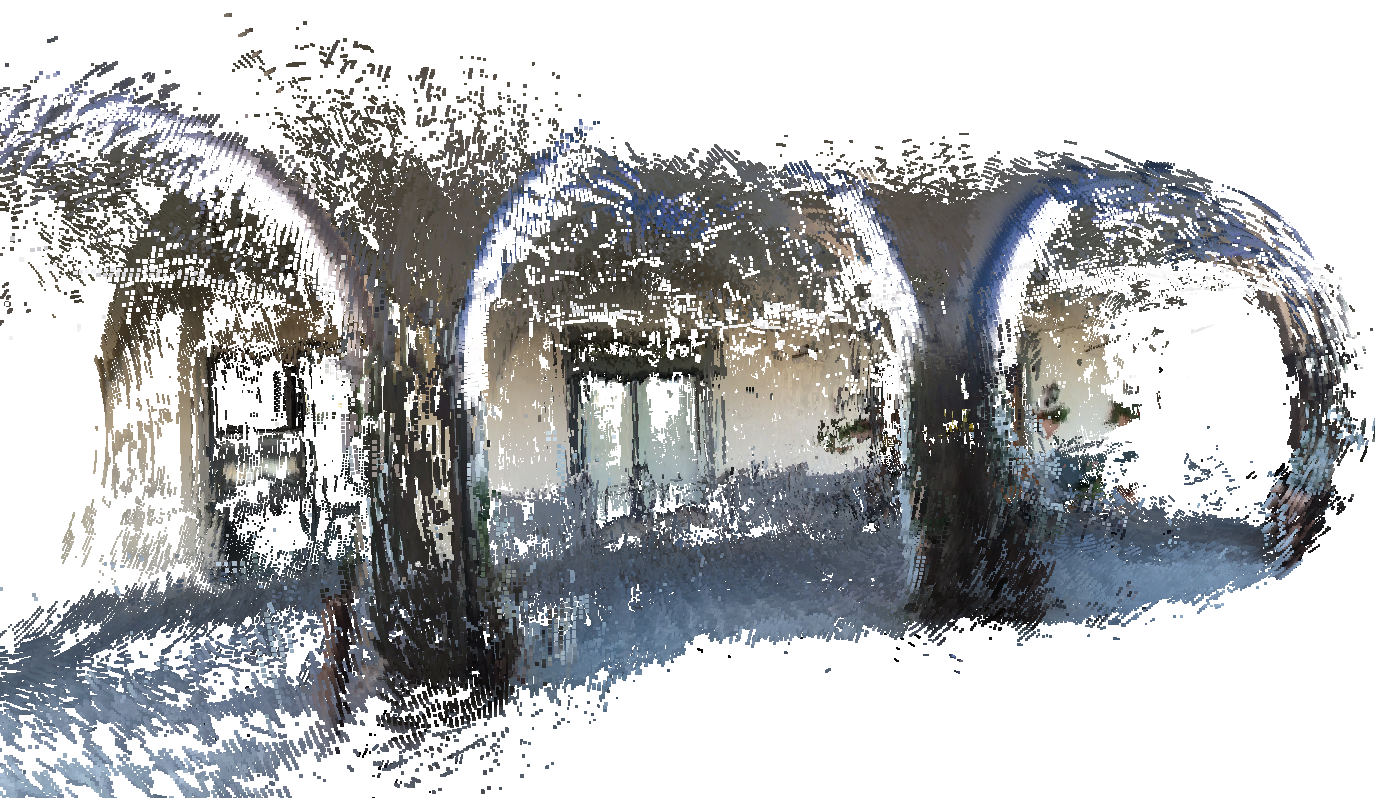
\includegraphics[width=\linewidth]{img/reconstruction00.png}
	\end{subfigure}
	%
	\begin{subfigure}{\linewidth}
		\centering
		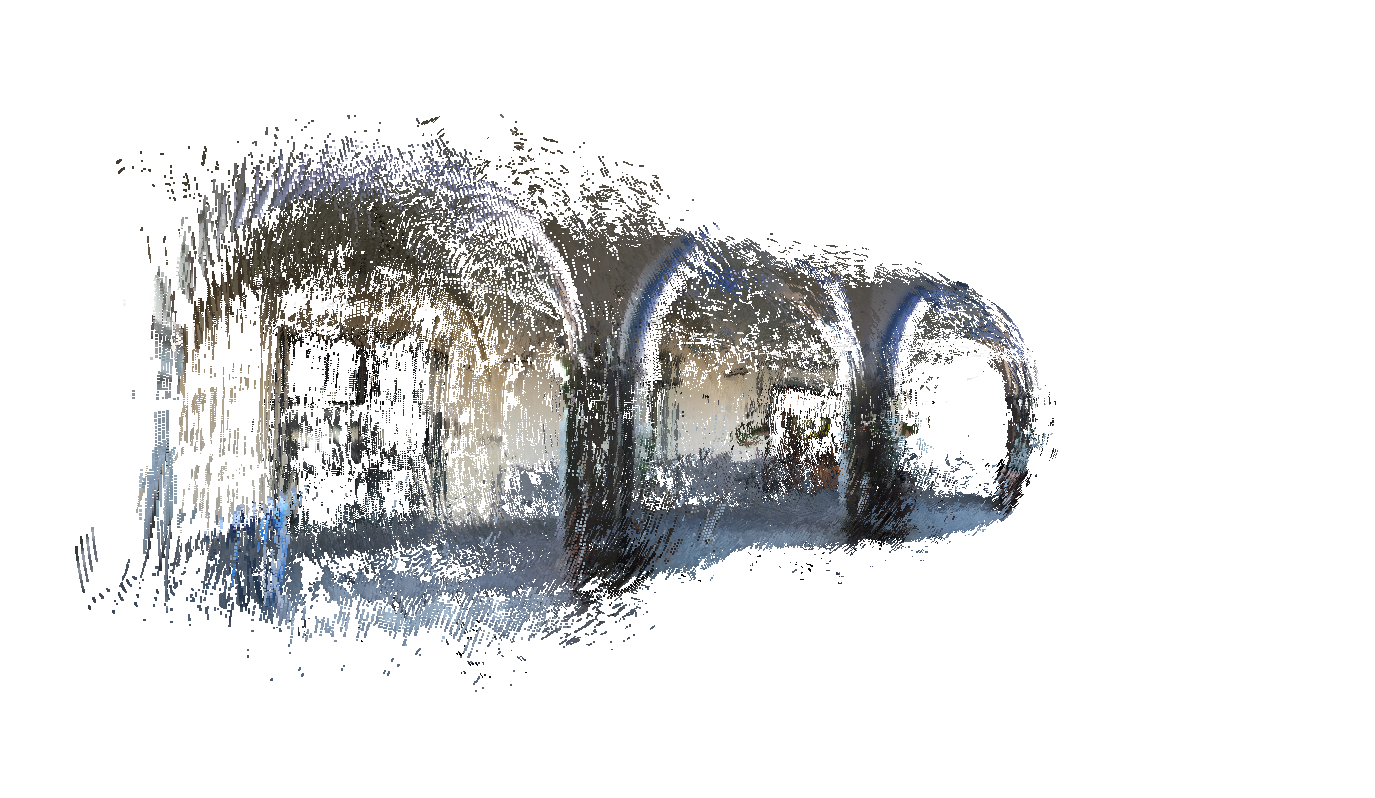
\includegraphics[width=\linewidth]{img/reconstruction01.png}
	\end{subfigure}
	\caption{Two views of the dense point cloud of the real town square
	(Section~\ref{subsec:real_environment}) obtained with our SfM pipeline.}
	\label{fig:real_reconstruction}
\end{figure}

\subsection{Limitations}\label{subsec:limitations}
As we expected, our pipeline fails when there are not enough feature points
that can be tracked in all the views of the window.
In the current implementation, there is no recovery procedure that deals with
this problem and we suggest some possible solutions in
Section~\ref{sec:future_work}.
